\documentclass{standalone}

\usepackage{graphicx}

\usepackage{tikz}

\usetikzlibrary{positioning}
\usetikzlibrary{arrows.meta}
\usetikzlibrary{calc}

\begin{document}

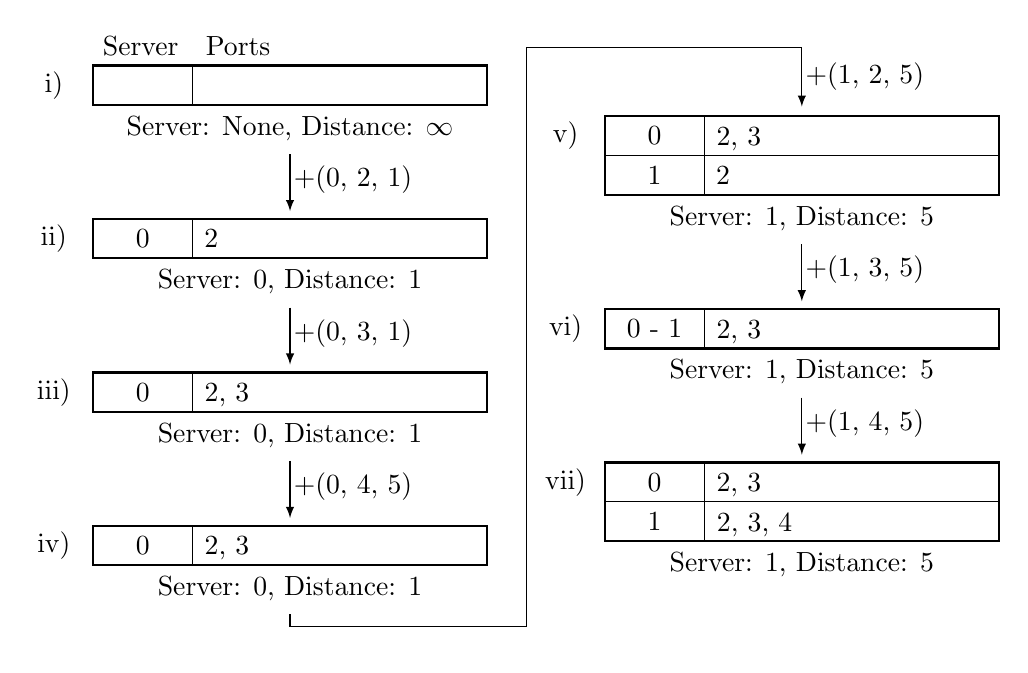
\begin{tikzpicture}[
    block/.style={align=center, rectangle, draw=black, fill=white, text width=16em}
]
    \node[] (T1) {Server};
    \node[] (T2) [right=0.1cm of T1] {Ports};

    % Empty figure
    \node[] (H1) at (T1.south west) {};
    \draw[thick] (H1) rectangle ($(H1)+(5,-.5)$);
    \draw ($(H1)+(1.26, 0.0)$) -- ($(H1)+(1.26,-.5)$);

    \node[] (I1) at ($(H1)+(-0.5, -.25)$) {i)};
    \node[] at ($(H1)+(2.5, -0.8)$) {Server: None, Distance: $\infty$};

    % After first addition
    \node[] (H2) [below=1.7cm of H1] {};
    \draw[thick] (H2) rectangle ($(H2)+(5,-.5)$);
    \draw ($(H2)+(1.26, 0.0)$) -- ($(H2)+(1.26,-.5)$);

    \node[] at ($(H2)+(0.63, -.25)$) {0};
    \node[] at ($(H2)+(1.5, -.25)$) {2};

    \node[] (I2) at ($(H2)+(-0.5, -.25)$) {ii)};
    \node[] at ($(H2)+(2.5, -0.8)$) {Server: 0, Distance: $1$};

    % After second addition
    \node[] (H3) [below=1.7cm of H2] {};
    \draw[thick] (H3) rectangle ($(H3)+(5,-.5)$);
    \draw ($(H3)+(1.26, 0.0)$) -- ($(H3)+(1.26,-.5)$);

    \node[] at ($(H3)+(0.63, -.25)$) {0};
    \node[] at ($(H3)+(1.7, -.29)$) {2, 3};

    \node[] (I2) at ($(H3)+(-0.5, -.25)$) {iii)};
    \node[] at ($(H3)+(2.5, -0.8)$) {Server: 0, Distance: $1$};

    % After third addition
    \node[] (H4) [below=1.7cm of H3] {};
    \draw[thick] (H4) rectangle ($(H4)+(5,-.5)$);
    \draw ($(H4)+(1.26, 0.0)$) -- ($(H4)+(1.26,-.5)$);

    \node[] at ($(H4)+(0.63, -.25)$) {0};
    \node[] at ($(H4)+(1.7, -.29)$) {2, 3};

    \node[] (I2) at ($(H4)+(-0.5, -.25)$) {iv)};
    \node[] at ($(H4)+(2.5, -0.8)$) {Server: 0, Distance: $1$};

    % New server
    \node[] (H5) at ($(H4)+(6.5, 5.2)$) {};
    \draw[thick] (H5) rectangle ($(H5)+(5,-1.0)$);
    \draw ($(H5)+(0, -0.5)$) -- ($(H5)+(5,-0.5)$);
    
    \draw ($(H5)+(1.26, 0.0)$) -- ($(H5)+(1.26,-1.0)$);

    \node[] at ($(H5)+(0.63, -.25)$) {0};
    \node[] at ($(H5)+(1.7, -.29)$) {2, 3};

    \node[] at ($(H5)+(0.63, -.75)$) {1};
    \node[] at ($(H5)+(1.5, -.75)$) {2};

    \node[] (I2) at ($(H5)+(-0.5, -.25)$) {v)};
    \node[] at ($(H5)+(2.5, -1.3)$) {Server: 1, Distance: $5$};

    % After second addition
    \node[] (H6) [below=2.2cm of H5] {};
    \draw[thick] (H6) rectangle ($(H6)+(5,-.5)$);
    \draw ($(H6)+(1.26, 0.0)$) -- ($(H6)+(1.26,-.5)$);

    \node[] at ($(H6)+(0.63, -.25)$) {0 - 1};
    \node[] at ($(H6)+(1.7, -.29)$) {2, 3};

    \node[] (I2) at ($(H6)+(-0.5, -.25)$) {vi)};
    \node[] at ($(H6)+(2.5, -0.8)$) {Server: 1, Distance: $5$};

    % After final addition
    \node[] (H7) [below=1.7cm of H6] {};
    \draw[thick] (H7) rectangle ($(H7)+(5,-1.0)$);
    \draw ($(H7)+(0, -0.5)$) -- ($(H7)+(5,-0.5)$);
    \draw ($(H7)+(1.26, 0.0)$) -- ($(H7)+(1.26,-1.0)$);

    \node[] at ($(H7)+(0.63, -.25)$) {0};
    \node[] at ($(H7)+(1.7, -.29)$) {2, 3};

    \node[] at ($(H7)+(0.63, -.75)$) {1};
    \node[] at ($(H7)+(1.9, -.79)$) {2, 3, 4};

    \node[] (I2) at ($(H7)+(-0.5, -.25)$) {vii)};
    \node[] at ($(H7)+(2.5, -1.3)$) {Server: 1, Distance: $5$};

    % Transition indications
    \node[] (T1) at ($(H1)+(2.5, -1)$) {};
    \draw[-latex] (T1) -- ($(H2) + (2.5, 0.1)$);
    \node[] at ($(T1)+(0.8, -0.45)$) {+(0, 2, 1)};

    \node[] (T2) at ($(H2)+(2.5, -1)$) {};
    \draw[-latex] (T2) -- ($(H3) + (2.5, 0.1)$);
    \node[] at ($(T2)+(0.8, -0.45)$) {+(0, 3, 1)};

    \node[] (T3) at ($(H3)+(2.5, -1)$) {};
    \draw[-latex] (T3) -- ($(H4) + (2.5, 0.1)$);
    \node[] at ($(T3)+(0.8, -0.45)$) {+(0, 4, 5)};

    \node[] (T4A) at ($(H4)+(2.5, -1)$) {};
    \node[] (T4B) at ($(H4)+(2.5, -1.4)$) {};
    \node[] (T4C) at ($(H5)+(-1, 1)$) {};
    \node[] (T4D) at ($(H5)+(2.5, 1)$) {};
    \node[] (T4E) at ($(H5)+(2.5, 0)$) {};
    \draw[] (T4A.south) -- (T4B.north) -| (T4C.south) -- (T4D.south);
    \draw[-latex] (T4D.south) -- (T4E.north);
    \node[] at ($(T4E)+(0.8, 0.5)$) {+(1, 2, 5)};

    \node[] (T5) at ($(H5)+(2.5, -1.5)$) {};
    \draw[-latex] (T5) -- ($(H6) + (2.5, 0.1)$);
    \node[] at ($(T5)+(0.8, -0.45)$) {+(1, 3, 5)};

    \node[] (T6) at ($(H6)+(2.5, -1)$) {};
    \draw[-latex] (T6) -- ($(H7) + (2.5, 0.1)$);
    \node[] at ($(T6)+(0.8, -0.45)$) {+(1, 4, 5)};
\end{tikzpicture}

\end{document}